% Options for packages loaded elsewhere
\PassOptionsToPackage{unicode}{hyperref}
\PassOptionsToPackage{hyphens}{url}
%
\documentclass[
  x11names]{article}
\usepackage{amsmath,amssymb}
\usepackage{lmodern}
\usepackage{iftex}
\ifPDFTeX
  \usepackage[T1]{fontenc}
  \usepackage[utf8]{inputenc}
  \usepackage{textcomp} % provide euro and other symbols
\else % if luatex or xetex
  \usepackage{unicode-math}
  \defaultfontfeatures{Scale=MatchLowercase}
  \defaultfontfeatures[\rmfamily]{Ligatures=TeX,Scale=1}
\fi
% Use upquote if available, for straight quotes in verbatim environments
\IfFileExists{upquote.sty}{\usepackage{upquote}}{}
\IfFileExists{microtype.sty}{% use microtype if available
  \usepackage[]{microtype}
  \UseMicrotypeSet[protrusion]{basicmath} % disable protrusion for tt fonts
}{}
\makeatletter
\@ifundefined{KOMAClassName}{% if non-KOMA class
  \IfFileExists{parskip.sty}{%
    \usepackage{parskip}
  }{% else
    \setlength{\parindent}{0pt}
    \setlength{\parskip}{6pt plus 2pt minus 1pt}}
}{% if KOMA class
  \KOMAoptions{parskip=half}}
\makeatother
\usepackage{xcolor}
\usepackage[margin=1in]{geometry}
\usepackage{graphicx}
\makeatletter
\def\maxwidth{\ifdim\Gin@nat@width>\linewidth\linewidth\else\Gin@nat@width\fi}
\def\maxheight{\ifdim\Gin@nat@height>\textheight\textheight\else\Gin@nat@height\fi}
\makeatother
% Scale images if necessary, so that they will not overflow the page
% margins by default, and it is still possible to overwrite the defaults
% using explicit options in \includegraphics[width, height, ...]{}
\setkeys{Gin}{width=\maxwidth,height=\maxheight,keepaspectratio}
% Set default figure placement to htbp
\makeatletter
\def\fps@figure{htbp}
\makeatother
\setlength{\emergencystretch}{3em} % prevent overfull lines
\providecommand{\tightlist}{%
  \setlength{\itemsep}{0pt}\setlength{\parskip}{0pt}}
\setcounter{secnumdepth}{-\maxdimen} % remove section numbering
\usepackage{fontspec} \usepackage{titling} \pretitle{\begin{center} \vspace{-3cm}
\includegraphics[width=\linewidth]{images/Base_info/logo.png}\LARGE\\} \posttitle{\end{center}} \usepackage{float} \usepackage{fancyhdr} \usepackage{ragged2e} \usepackage{caption} \usepackage{colortbl} \captionsetup[figure]{labelformat=empty} \arrayrulecolor{white} \pagestyle{fancy} \fancyhead[L,C]{} \fancypagestyle{plain}{\pagestyle{fancy}} \PassOptionsToPackage{dvipsnames,svgnames*,x11names*}{xcolor} \definecolor{ceil}{rgb}{0.57, 0.63, 0.81} \usepackage[export]{adjustbox} \usepackage{wrapfig} \usepackage{graphicx} \usepackage{caption}
\usepackage{booktabs}
\usepackage{longtable}
\usepackage{array}
\usepackage{multirow}
\usepackage{wrapfig}
\usepackage{float}
\usepackage{colortbl}
\usepackage{pdflscape}
\usepackage{tabu}
\usepackage{threeparttable}
\usepackage{threeparttablex}
\usepackage[normalem]{ulem}
\usepackage{makecell}
\usepackage{xcolor}
\ifLuaTeX
  \usepackage{selnolig}  % disable illegal ligatures
\fi
\IfFileExists{bookmark.sty}{\usepackage{bookmark}}{\usepackage{hyperref}}
\IfFileExists{xurl.sty}{\usepackage{xurl}}{} % add URL line breaks if available
\urlstyle{same} % disable monospaced font for URLs
\hypersetup{
  hidelinks,
  pdfcreator={LaTeX via pandoc}}

\author{}
\date{\vspace{-2.5em}Fecha de creación: 03 April, 2023}

\begin{document}

\setmainfont{Arial}
\setsansfont{Arial}
\setmonofont{Arial}

\newcommand\invisiblesection[1]{%
  \refstepcounter{section}%
  \addcontentsline{toc}{section}{\protect\numberline{\thesection}#1}%
  \sectionmark{#1}}

\fancyhead[R]{\textbf{http://doi.org/10.31687/SaremLR.19.205}}

%
  \refstepcounter{section}%
  \addcontentsline{toc}{section}{\protect\numberline{\thesection}GENERALIDADES}%
  \sectionmark{GENERALIDADES}
\vspace{-0.4cm}


\includegraphics[width=1\linewidth]{images/Base_info/logo}

\vspace{1cm}

\begin{minipage}{0.7\textwidth}
\vspace{0.3cm}
\fontsize{20}{24}\selectfont\textit{Lama guanicoe}

\vspace{0.3cm}
\fontsize{30}{36}\selectfont Guanaco
\end{minipage}
\hspace{0.05\textwidth}
\begin{minipage}{0.25\textwidth}

\includegraphics[width=\textwidth]{images/lc.png}
\end{minipage}

\normalsize

\begin{figure}[H]

{\centering 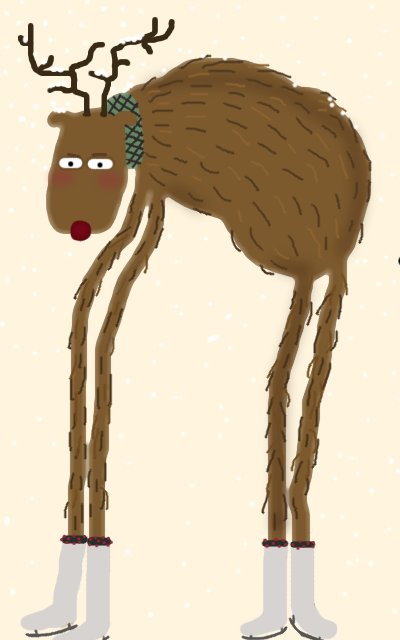
\includegraphics[width=0.35\linewidth]{photos/Blastocerus dichotomus} 

}

\caption{Fotos por Salvador Dali}\label{fig:image}
\end{figure}

\begin{center}\rule{0.5\linewidth}{0.5pt}\end{center}

\justifying

\textbf{Citar como:} Carmanchahi, Pablo D.; Panebianco, Antonella;
Leggieri, Leonardo; Barri, Fernando; Marozzi, Antonela; Flores, Celina;
Moreno, Pablo; Schroeder, Natalia; Cepeda, Carla; Oliva, Gabriel; Kin,
Marta Susana; Gregorio, Pablo; Ovejero, Ramiro; Acebes, Pablo;
Schneider, Cristian F.; Pedrana, Julieta; Taraborelli, Paula. (2019).
\emph{Lama guanicoe}. En: SAyDS--SAREM (eds.) Categorización 2019 de los
mamíferos de Argentina según su riesgo de extinción. Lista Roja de los
mamíferos de Argentina. \url{http://doi.org/10.31687/SaremLR.19.205}

\begin{center}\rule{0.5\linewidth}{0.5pt}\end{center}

\newpage

%
  \refstepcounter{section}%
  \addcontentsline{toc}{section}{\protect\numberline{\thesection}ÁREA DE DISTRIBUCIÓN ACTUAL}%
  \sectionmark{ÁREA DE DISTRIBUCIÓN ACTUAL}
\begin{table}[H]
\centering
\begin{tabular}[t]{>{\raggedright\arraybackslash}m{16cm}>{}m{16cm}}
\toprule
\cellcolor{ceil}{\textcolor{white}{\textbf{\rule{0pt}{14pt}ÁREA DE DISTRIBUCIÓN ACTUAL}}}\\
\bottomrule
\end{tabular}
\end{table}

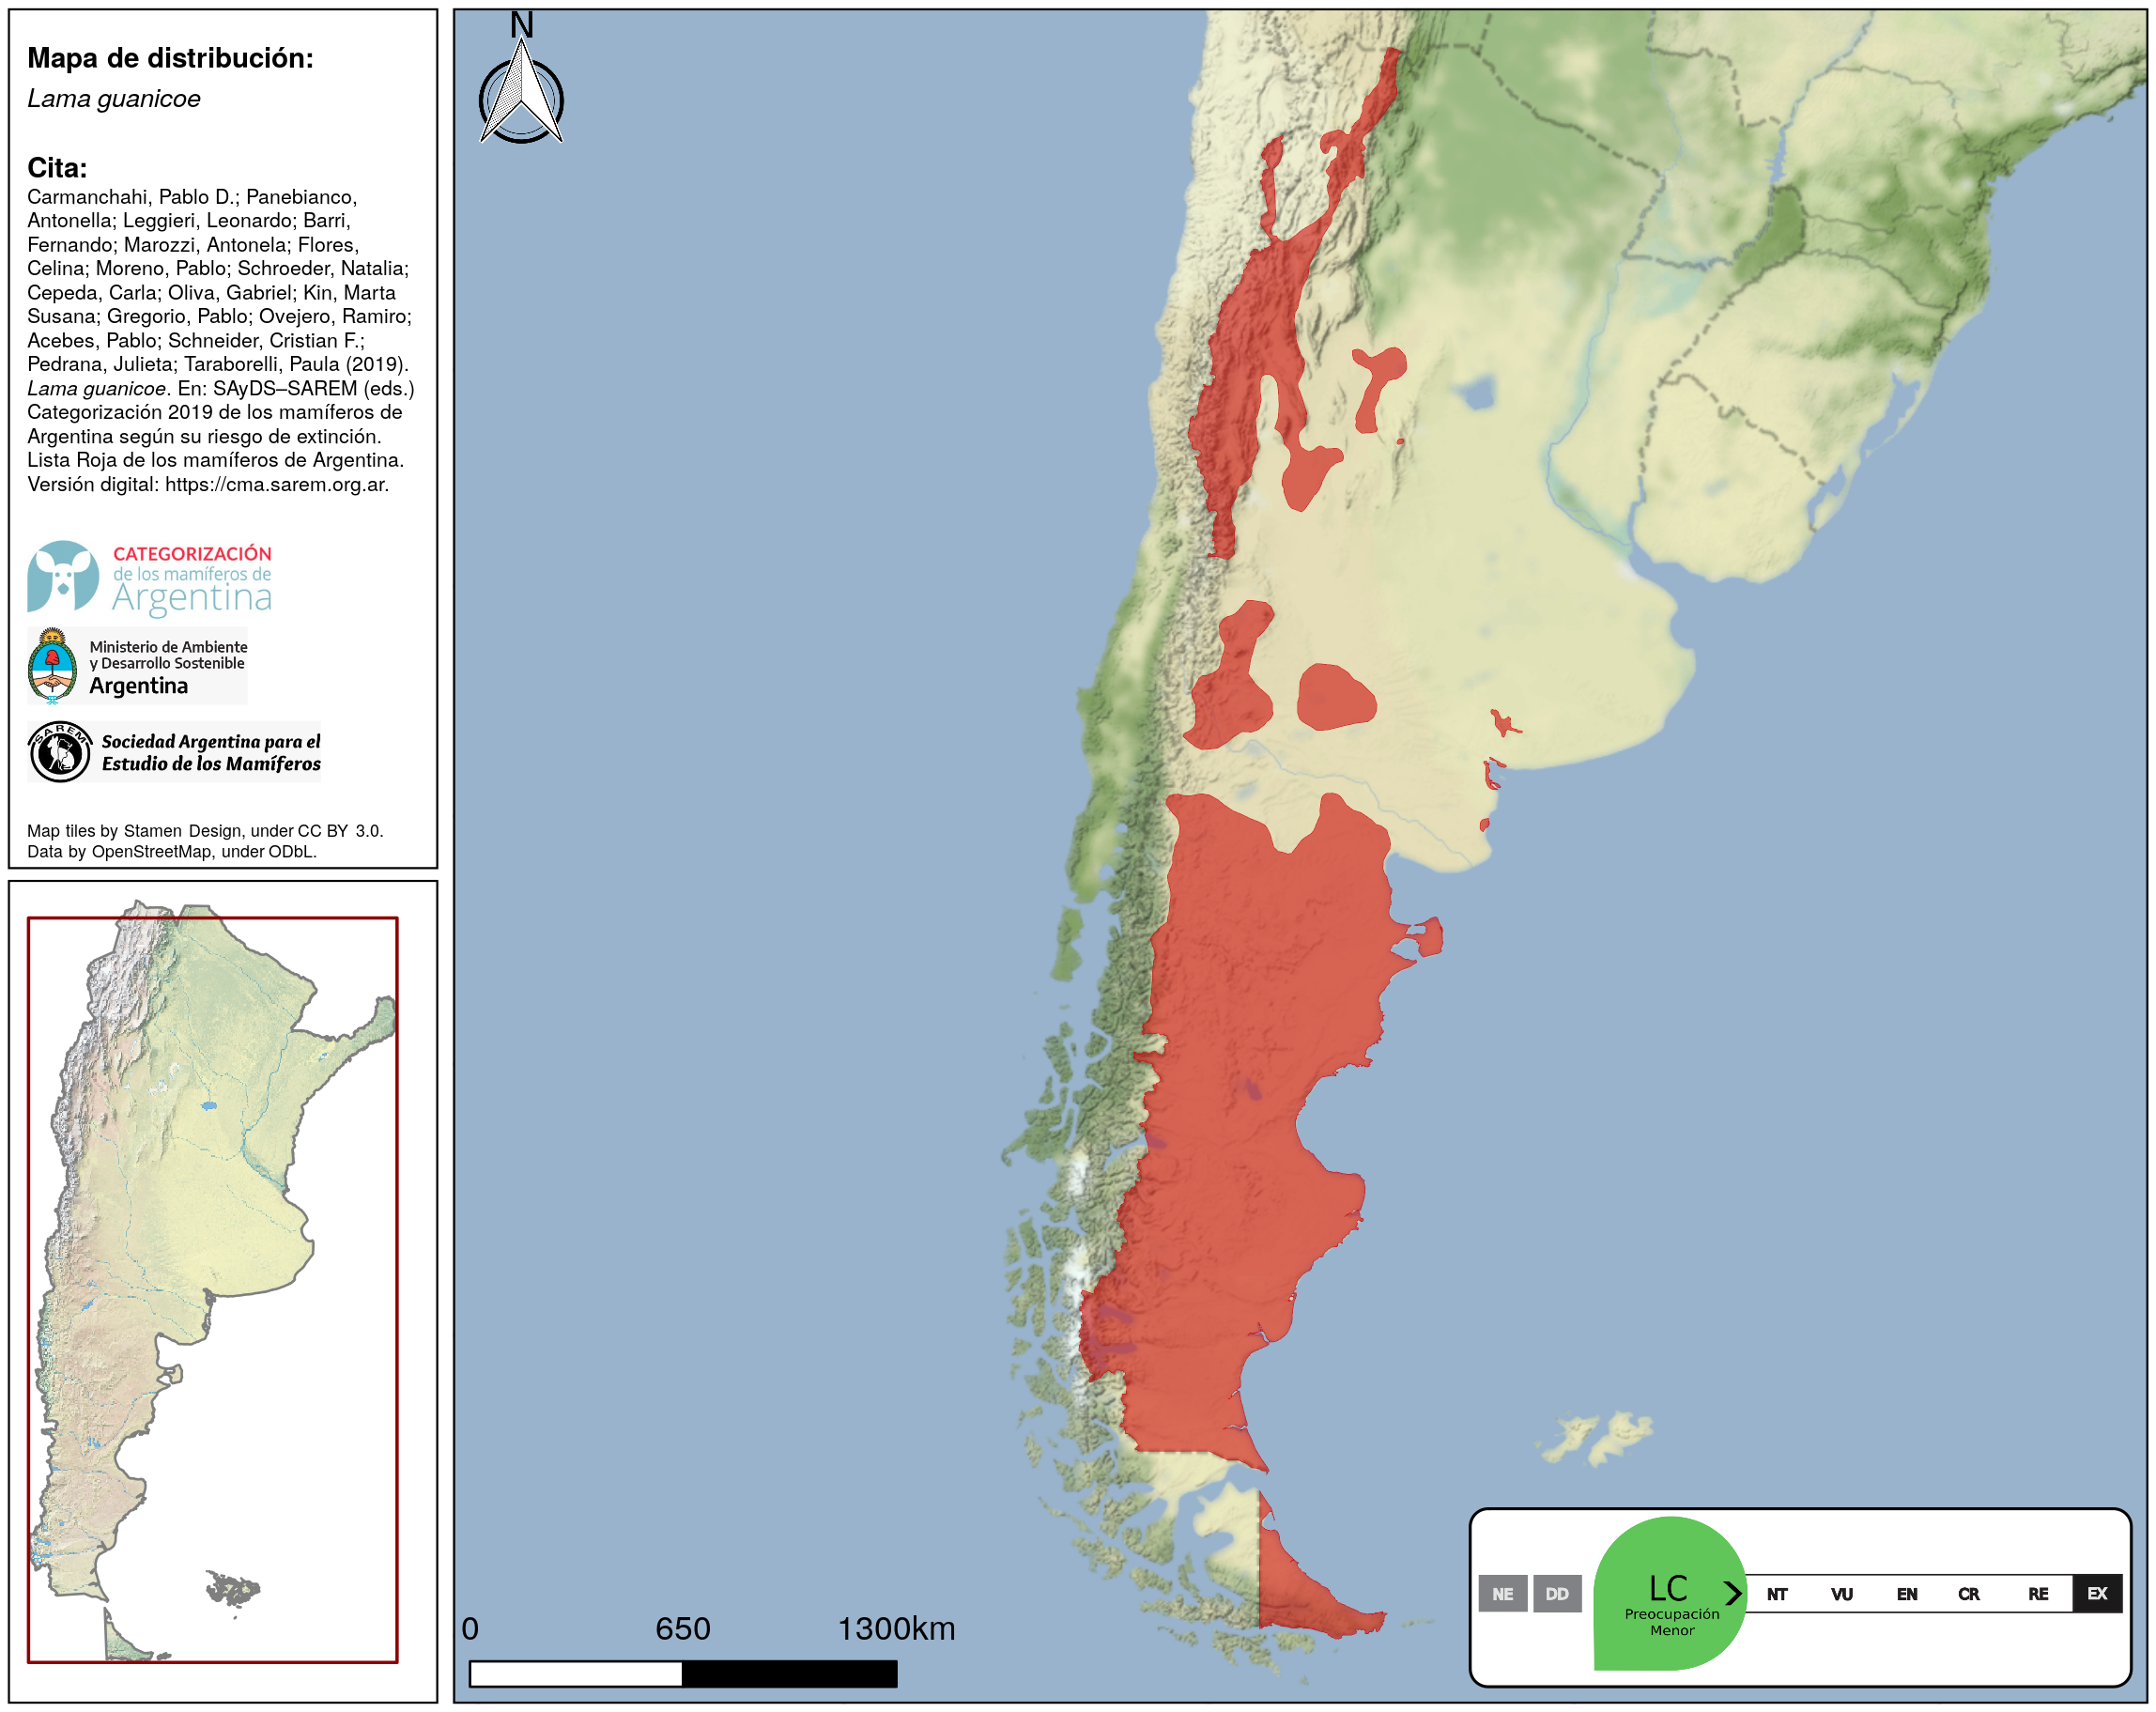
\includegraphics[width=1\linewidth]{maps/Cetartiodactyla/Lama_guanicoe}

%
  \refstepcounter{section}%
  \addcontentsline{toc}{section}{\protect\numberline{\thesection}CATEGORÍAS DE CONSERVACIÓN}%
  \sectionmark{CATEGORÍAS DE CONSERVACIÓN}
\begin{table}[H]
\centering
\begin{tabular}[t]{>{\raggedright\arraybackslash}m{16cm}>{}m{16cm}}
\toprule
\cellcolor{ceil}{\textcolor{white}{\textbf{\rule{0pt}{14pt}CATEGORÍAS DE CONSERVACIÓN}}}\\
\bottomrule
\end{tabular}
\end{table}

\vspace{-0.4cm}

\textbf{Categoría Nacional de Conservación 2019}

LC (Preocupación Menor)

\textbf{Criterios y subcriterios}

NA

\textbf{Justificación de la categorización}

Si bien hubo una drástica reducción poblacional del guanaco en
Argentina, estimada entre el 90 y 97\% desde la colonización europea, la
tendencia de los últimos 30 años fue en aumento (González \& Acebes
2016). Actualmente, la población total estimada para Argentina es de un
poco menos de un millón de guanacos (González \& Acebes 2016) y la
amplitud en la extensión de presencia y en el área de ocupación sugiere
que la especie a nivel nacional sea catalogada como de Preocupación
Menor (LC). Sin embargo, esta categorización debe tomarse con cautela,
puesto que si bien las poblaciones en Patagonia se han incrementado
durante la última década, las del centro-oeste y norte del país, son
poblaciones reducidas, fragmentadas y aisladas. Por lo tanto, es
necesario evaluar el estado de conservación a nivel regional (ver
evaluación de sub-poblaciones).

\textbf{Evaluación de subpoblaciones locales}

\begin{tabu} to \linewidth {>{\raggedright}X>{\raggedright}X>{\raggedright}X}
\toprule
\textbf{Subpoblación} & \textbf{Categoría} & \textbf{Criterios y subcriterios}\\
\arrayrulecolor{white}
\midrule
\cellcolor{gray!6}{de la Puna y peri Puna (San Juan, La Rioja, Catamarca, Tucuman, Jujuy, Salta)} & \cellcolor{gray!6}{EN (En Peligro)} & \cellcolor{gray!6}{B1ab(iii)}\\
\bottomrule
\end{tabu}

\textbf{Justificación}

En toda la región, se estima que hay unos 18.000 - 20.000~individuos
distribuidos mayormente en sub-poblaciones fragmentadas y en superficies
acotadas (Baigún et al.~2008). Por ejemplo, la subpoblación del Parque
Provincial Ischigualasto (San Juan) y Parque Nacional~Talampaya (La
Rioja) consta de unos 500 individuos (Acebes et al.~2010), en un área
aproximada de 2.800 Km2. Las sub-poblaciones de Jujuy, Salta y Tucumán
son de pequeño tamaño (\textless{} 700 individuos; {[}Baigún et
al.~2008{]}), están restringidas a sitios aislados y están desconectadas
espacialmente. La mayor proporción de estas sub-poblaciones se encuentra
en San Juan (74\%), Catamarca (10\%) y La Rioja (9\%) (Baigún et
al.~2008). La principal amenaza en estas zonas es la cacería furtiva. La
principal amenaza en estas zonas es la cacería furtiva.

Por lo tanto, se estima que la extensión de presencia (EOO) es
\textless{} 5.000 Km2, está severamente fragmentada y hay
una~disminución continua observada de la extensión de presencia y/o
calidad del hábitat,~número de localidades o subpoblaciones y en número
de individuos maduros.\vspace{0.5cm}

\begin{tabu} to \linewidth {>{\raggedright}X>{\raggedright}X>{\raggedright}X}
\toprule
\textbf{Subpoblación} & \textbf{Categoría} & \textbf{Criterios y subcriterios}\\
\arrayrulecolor{white}
\midrule
\cellcolor{gray!6}{Chaqueña (centro-norte de Córdoba)} & \cellcolor{gray!6}{CR (En Peligro Crítico)} & \cellcolor{gray!6}{B1ab(iii)}\\
\bottomrule
\end{tabu}

\textbf{Justificación}

La sub-población de guanacos chaqueños se encuentra restringida a un
área muy reducida de lo que fuera su distribución original, aislada de
otras subpoblaciones (Costa \& Barri 2018; Geisa et al.~2018). Enfrenta
la amenaza de la pérdida de hábitat y cacería furtiva. Se estima que
esta sub-población no supera los 100 individuos (Barri F.,~obs. pers.).
Por lo tanto, se calcula que la extensión de presencia (EOO) es
\textless{} 100 Km2, está severamente fragmentada y hay una disminución
continua observada de la extensión de presencia y/o calidad del hábitat,
número de localidades o subpoblaciones y en número de individuos
maduros.\vspace{0.5cm}

\begin{tabu} to \linewidth {>{\raggedright}X>{\raggedright}X>{\raggedright}X}
\toprule
\textbf{Subpoblación} & \textbf{Categoría} & \textbf{Criterios y subcriterios}\\
\arrayrulecolor{white}
\midrule
\cellcolor{gray!6}{Patagonia Norte-Centro (Mendoza, Neuquén, Río Negro, Chubut)} & \cellcolor{gray!6}{LC (Preocupación Menor)} & \cellcolor{gray!6}{Dentro del rango de distribución de este camélido, la población de La Payunia (sur de Mendoza) destaca como una de las más abundantes y resulta la más grande de la región cuyana. Los guanacos en La Payunia cambian notablemente su distribución espacial a lo largo del año debido a su carácter migratorio. En la zona norte del área protegida se distribuyen ampliamente alrededor de 26.000 guanacos durante primavera- verano, mientras que en invierno pueden permanecer en la zona menos de 4.000 guanacos debido a los desplazamientos temporales que realizan hacia otros sectores de la Reserva y los alrededores (Schroeder et al. 2014; Bolgeri 2016). En la provincia de Chubut se muestrearon el 76\% de las rutas disponibles (7.000 km) en la temporada reproductiva del 2016 (Pedrana et al. en prensa). A partir de estos muestreos, se estimó una población total de guanacos de 657.304 individuos (95\% CI 457.437 a 944.059 individuos), que representa una densidad media de 2,97 ind/Km2. Asimismo en áreas consideradas con hábitat marginal para el guanaco la densidad promedio fue de 0,49 ind/Km2, mientras que en los hábitats considerados moderados y adecuados para la especie, las densidades fueron 2,74 y 3,93 ind/Km2, respectivamente.}\\
\bottomrule
\end{tabu}

\textbf{Justificación}

Patagonia Sur (Santa Cruz)

Subpoblación

Dentro del rango de distribución de este camélido, la población de La
Payunia (sur de Mendoza) destaca como una de las más abundantes y
resulta la más grande de la región cuyana. Los guanacos en La Payunia
cambian notablemente su distribución espacial a lo largo del año debido
a su carácter migratorio. En la zona norte del área protegida se
distribuyen ampliamente alrededor de 26.000 guanacos durante primavera-
verano, mientras que en invierno pueden permanecer en la zona menos de
4.000 guanacos debido a los desplazamientos temporales que realizan
hacia otros sectores de la Reserva y los alrededores (Schroeder et
al.~2014; Bolgeri 2016). En la provincia de Chubut se muestrearon el
76\% de las rutas disponibles (7.000 km) en la temporada reproductiva
del 2016 (Pedrana et al.~en prensa). A partir de estos muestreos, se
estimó una población total de guanacos de 657.304 individuos (95\% CI
457.437 a 944.059 individuos), que representa una densidad media de 2,97
ind/Km2. Asimismo en áreas consideradas con hábitat marginal para el
guanaco la densidad promedio fue de 0,49 ind/Km2, mientras que en los
hábitats considerados moderados y adecuados para la especie, las
densidades fueron 2,74 y 3,93 ind/Km2, respectivamente.\vspace{0.5cm}

\begin{tabu} to \linewidth {>{\raggedright}X>{\raggedright}X>{\raggedright}X}
\toprule
\textbf{Subpoblación} & \textbf{Categoría} & \textbf{Criterios y subcriterios}\\
\arrayrulecolor{white}
\midrule
\cellcolor{gray!6}{Patagonia Sur (Santa Cruz)} & \cellcolor{gray!6}{LC (Preocupación Menor)} & \cellcolor{gray!6}{A partir de censos de vehículo, donde se recorrió 8.141 km de rutas (93\% de las rutas disponibles) en la provincia de Santa Cruz, se estimó que la densidad media de guanacos era de 4.79 ind/Km2, con un coeficientes de variación del 20\% (Travaini et al. 2015). Las densidades poblacionales estimadas aumentan según las categorías de hábitat consideradas (Hábitat marginal, moderado y adecuado) (Travaini et al. 2007; Pedrana et al. 2010). Con lo cual, la densidad media se estimó en 1,12 ind/Km2 en zonas con hábitat marginal para la especie hasta una densidad media de 7,74 ind/Km2 en áreas con hábitat adecuados para la misma. A partir del cálculo de estas densidades y teniendo en cuenta las categorías de hábitat definidas por Pedrana et al. (2010), se calculó que la población total de guanacos para Santa Cruz era de 1.066.600 individuos (95\% CI 727.800-1.563.200).}\\
\bottomrule
\end{tabu}

\textbf{Justificación}

Fueguina (porción Argentina de la Isla Grande de Tierra del Fuego)

Subpoblación

A partir de censos de vehículo, donde se recorrió 8.141 km de rutas
(93\% de las rutas disponibles) en la provincia de Santa Cruz, se estimó
que la densidad media de guanacos era de 4.79 ind/Km2, con un
coeficientes de variación del 20\% (Travaini et al.~2015). Las
densidades poblacionales estimadas aumentan según las categorías de
hábitat consideradas (Hábitat marginal, moderado y adecuado) (Travaini
et al.~2007; Pedrana et al.~2010). Con lo cual, la densidad media se
estimó en 1,12 ind/Km2 en zonas con hábitat marginal para la especie
hasta una densidad media de 7,74 ind/Km2 en áreas con hábitat adecuados
para la misma. A partir del cálculo de estas densidades y teniendo en
cuenta las categorías de hábitat definidas por Pedrana et al.~(2010), se
calculó que la población total de guanacos para Santa Cruz era de
1.066.600 individuos (95\% CI 727.800-1.563.200).\vspace{0.5cm}

\begin{tabu} to \linewidth {>{\raggedright}X>{\raggedright}X>{\raggedright}X}
\toprule
\textbf{Subpoblación} & \textbf{Categoría} & \textbf{Criterios y subcriterios}\\
\arrayrulecolor{white}
\midrule
\cellcolor{gray!6}{Fueguina (porción Argentina de la Isla Grande de Tierra del Fuego)} & \cellcolor{gray!6}{LC (Preocupación Menor)} & \cellcolor{gray!6}{La distribución actual de la especie en la región parece coincidir con la descripta para el año 1995 (datos no publicados), en la cual, la mayor concentración de individuos se localizó al centro de la Isla (Región Ecotono Bosque-Estepa) (Montes et al. 2000). En esta zona, se estima que la abundancia varía entre los 23.000-33.000 individuos, según la época del año (no reproductiva-reproductiva, respectivamente) (Flores et al. 2018). Las densidades promedios para las mismas épocas variaron de 3 a 5 ind/Km2.}\\
\bottomrule
\end{tabu}

\textbf{Justificación}

Buenos Aires y La Pampa

Subpoblación

La distribución actual de la especie en la región parece coincidir con
la descripta para el año 1995 (datos no publicados), en la cual, la
mayor concentración de individuos se localizó al centro de la Isla
(Región Ecotono Bosque-Estepa) (Montes et al.~2000). En esta zona, se
estima que la abundancia varía entre los 23.000-33.000 individuos, según
la época del año (no reproductiva-reproductiva, respectivamente) (Flores
et al.~2018). Las densidades promedios para las mismas épocas variaron
de 3 a 5 ind/Km2.\vspace{0.5cm}

\begin{tabu} to \linewidth {>{\raggedright}X>{\raggedright}X>{\raggedright}X}
\toprule
\textbf{Subpoblación} & \textbf{Categoría} & \textbf{Criterios y subcriterios}\\
\arrayrulecolor{white}
\midrule
\cellcolor{gray!6}{Buenos Aires y La Pampa} & \cellcolor{gray!6}{CR (En Peligro Crítico)} & \cellcolor{gray!6}{NA}\\
\bottomrule
\end{tabu}

\textbf{Justificación}

NA

NA

NA

NA

CR (En Peligro Crítico)

\textbf{Categoría Res. SAyDS 1030/04}

NA (No Amenazada)

\textbf{Categorías nacionales de conservación previas (SAREM)}

\arrayrulecolor{white}

%
  \refstepcounter{section}%
  \addcontentsline{toc}{section}{\protect\numberline{\thesection}TAXONOMÍA Y NOMENCLATURA}%
  \sectionmark{TAXONOMÍA Y NOMENCLATURA}
\begin{table}[H]
\centering
\begin{tabular}[t]{>{\raggedright\arraybackslash}m{16cm}>{}m{16cm}}
\toprule
\cellcolor{ceil}{\textcolor{white}{\textbf{\rule{0pt}{14pt}TAXONOMÍA Y NOMENCLATURA}}}\\
\bottomrule
\end{tabular}
\end{table}

%
  \refstepcounter{section}%
  \addcontentsline{toc}{section}{\protect\numberline{\thesection}INFORMACIÓN RELEVANTE PARA LA EVALUACIÓN}%
  \sectionmark{INFORMACIÓN RELEVANTE PARA LA EVALUACIÓN}
\begin{table}[H]
\centering
\begin{tabular}[t]{>{\raggedright\arraybackslash}m{16cm}>{}m{16cm}}
\toprule
\cellcolor{ceil}{\textcolor{white}{\textbf{\rule{0pt}{14pt}INFORMACIÓN RELEVANTE PARA LA EVALUACIÓN}}}\\
\bottomrule
\end{tabular}
\end{table}

%
  \refstepcounter{section}%
  \addcontentsline{toc}{section}{\protect\numberline{\thesection}RANGO GEOGRÁFICO, OCURRENCIA Y ABUNDANCIA Y NOMENCLATURA}%
  \sectionmark{RANGO GEOGRÁFICO, OCURRENCIA Y ABUNDANCIA Y NOMENCLATURA}
\begin{table}[H]
\centering
\begin{tabular}[t]{>{\raggedright\arraybackslash}m{16cm}>{}m{16cm}}
\toprule
\cellcolor{ceil}{\textcolor{white}{\textbf{\rule{0pt}{14pt}RANGO GEOGRÁFICO, OCURRENCIA Y ABUNDANCIA Y NOMENCLATURA}}}\\
\bottomrule
\end{tabular}
\end{table}

%
  \refstepcounter{section}%
  \addcontentsline{toc}{section}{\protect\numberline{\thesection}DATOS MORFOMÉTRICOS}%
  \sectionmark{DATOS MORFOMÉTRICOS}
\begin{table}[H]
\centering
\begin{tabular}[t]{>{\raggedright\arraybackslash}m{16cm}>{}m{16cm}}
\toprule
\cellcolor{ceil}{\textcolor{white}{\textbf{\rule{0pt}{14pt}DATOS MORFOMÉTRICOS}}}\\
\bottomrule
\end{tabular}
\end{table}

%
  \refstepcounter{section}%
  \addcontentsline{toc}{section}{\protect\numberline{\thesection}RASGOS ETO-ECOLÓGICOS}%
  \sectionmark{RASGOS ETO-ECOLÓGICOS}
\begin{table}[H]
\centering
\begin{tabular}[t]{>{\raggedright\arraybackslash}m{16cm}>{}m{16cm}}
\toprule
\cellcolor{ceil}{\textcolor{white}{\textbf{\rule{0pt}{14pt}RASGOS ETO-ECOLÓGICOS}}}\\
\bottomrule
\end{tabular}
\end{table}

%
  \refstepcounter{section}%
  \addcontentsline{toc}{section}{\protect\numberline{\thesection}CONSERVACIÓN E INVESTIGACIÓN}%
  \sectionmark{CONSERVACIÓN E INVESTIGACIÓN}
\begin{table}[H]
\centering
\begin{tabular}[t]{>{\raggedright\arraybackslash}m{16cm}>{}m{16cm}}
\toprule
\cellcolor{ceil}{\textcolor{white}{\textbf{\rule{0pt}{14pt}CONSERVACIÓN E INVESTIGACIÓN}}}\\
\bottomrule
\end{tabular}
\end{table}

%
  \refstepcounter{section}%
  \addcontentsline{toc}{section}{\protect\numberline{\thesection}BIBLIOGRAFÍA}%
  \sectionmark{BIBLIOGRAFÍA}
\begin{table}[H]
\centering
\begin{tabular}[t]{>{\raggedright\arraybackslash}m{16cm}>{}m{16cm}}
\toprule
\cellcolor{ceil}{\textcolor{white}{\textbf{\rule{0pt}{14pt}BIBLIOGRAFÍA}}}\\
\bottomrule
\end{tabular}
\end{table}

\newpage

%
  \refstepcounter{section}%
  \addcontentsline{toc}{section}{\protect\numberline{\thesection}AUTORES}%
  \sectionmark{AUTORES}
\begin{table}[H]
\centering
\begin{tabular}[t]{>{\raggedright\arraybackslash}m{16cm}>{}m{16cm}}
\toprule
\cellcolor{ceil}{\textcolor{white}{\textbf{\rule{0pt}{14pt}AUTORES}}}\\
\bottomrule
\end{tabular}
\end{table}

\textbf{AUTORES}

\begin{tabu} to \linewidth {>{}l>{\raggedright\arraybackslash}p{2cm}>{\raggedright}X}
\toprule
\textbf{\cellcolor{gray!6}{Acebes, Pablo}} & \cellcolor{gray!6}{} & \cellcolor{gray!6}{Universidad Autónoma de Madrid, , España}\\
\textbf{Barri, Fernando} &  & Instituto de Diversidad y Ecología Animal (IDEA), CONICET-Universidad Nacional de Córdoba, Córdoba, Argentina\\
\textbf{\cellcolor{gray!6}{Carmanchahi, Pablo D.}} & \cellcolor{gray!6}{} & \cellcolor{gray!6}{Grupo de Investigaciones en Eco-Fisiología de Fauna Silvestre (GIEFAS), Instituto Nacional de Investigaciones en Biodiversidad y Medio Ambiente (INIBIOMA), Asentamiento Universitario San Martín de los Andes - Universidad Nacional del Comahue - CONICET, San Martín de los Andes, Neuquén, Argentina}\\
\textbf{Cepeda, Carla} &  & EEA-Santa Cruz, Instituto Nacional de Tecnología Agropecuaria (INTA), Río Gallegos, Santa Cruz, Argentina\\
\textbf{\cellcolor{gray!6}{Flores, Celina}} & \cellcolor{gray!6}{} & \cellcolor{gray!6}{Centro Austral de Investigaciones Científicas y Técnicas (CADIC-CONICET), Ushuaia, Tierra del Fuego, Argentina}\\
\addlinespace
\textbf{Gregorio, Pablo} &  & Grupo de Investigaciones en Eco-Fisiología de Fauna Silvestre (GIEFAS), Instituto Nacional de Investigaciones en Biodiversidad y Medio Ambiente (INIBIOMA), Asentamiento Universitario San Martín de los Andes - Universidad Nacional del Comahue - CONICET, San Martín de los Andes, Neuquén, Argentina\\
\textbf{\cellcolor{gray!6}{Kin, Marta Susana}} & \cellcolor{gray!6}{} & \cellcolor{gray!6}{Facultad de Ciencias Exactas y Naturales, Universidad Nacional de La Pampa, Santa Rosa, La Pampa, Argentina}\\
\textbf{Leggieri, Leonardo} &  & Grupo de Investigaciones en Eco-Fisiología de Fauna Silvestre (GIEFAS), Instituto Nacional de Investigaciones en Biodiversidad y Medio Ambiente (INIBIOMA), Asentamiento Universitario San Martín de los Andes - Universidad Nacional del Comahue - CONICET, San Martín de los Andes, Neuquén, Argentina\\
\textbf{\cellcolor{gray!6}{Marozzi, Antonela}} & \cellcolor{gray!6}{} & \cellcolor{gray!6}{Grupo de Investigaciones en Eco-Fisiología de Fauna Silvestre (GIEFAS), Instituto Nacional de Investigaciones en Biodiversidad y Medio Ambiente (INIBIOMA), Asentamiento Universitario San Martín de los Andes - Universidad Nacional del Comahue - CONICET, San Martín de los Andes, Neuquén, Argentina}\\
\textbf{Moreno, Pablo} &  & Grupo de Investigaciones de la Biodiversidad (GiB), Instituto Argentino de Investigaciones de Zonas Aridas (IADIZA), CCT CONICET Mendoza, Mendoza, Argentina\\
\addlinespace
\textbf{\cellcolor{gray!6}{Oliva, Gabriel}} & \cellcolor{gray!6}{} & \cellcolor{gray!6}{EEA-Santa Cruz, Instituto Nacional de Tecnología Agropecuaria (INTA), Río Gallegos, Santa Cruz, Argentina}\\
\textbf{Ovejero, Ramiro} &  & Instituto de Ecología Regional (IER), Universidad Nacional de Tucumán - CONICET, Yerba Buena, Tucumán, Argentina\\
\textbf{\cellcolor{gray!6}{Panebianco, Antonella}} & \cellcolor{gray!6}{} & \cellcolor{gray!6}{Grupo de Investigaciones en Eco-Fisiología de Fauna Silvestre (GIEFAS), Instituto Nacional de Investigaciones en Biodiversidad y Medio Ambiente (INIBIOMA), Asentamiento Universitario San Martín de los Andes - Universidad Nacional del Comahue - CONICET, San Martín de los Andes, Neuquén, Argentina}\\
\textbf{Pedrana, Julieta} &  & Grupo de Recursos Naturales y Gestión Ambiental, Instituto Nacional de Tecnología Agropecuaria (INTA), Balcarce, Buenos Aires, Argentina\\
\textbf{\cellcolor{gray!6}{Schneider, Cristian F.}} & \cellcolor{gray!6}{} & \cellcolor{gray!6}{Asociación para la Conservación y Estudio de la Naturaleza (ACEN), Córdoba, Argentina}\\
\addlinespace
\textbf{Schroeder, Natalia} &  & Instituto Argentino de Investigaciones de las Zonas Áridas (IADIZA), CCT Mendoza - CONICET, Mendoza, Argentina\\
\textbf{\cellcolor{gray!6}{Taraborelli, Paula}} & \cellcolor{gray!6}{} & \cellcolor{gray!6}{EEA-Barrow, Instituto Nacional de Tecnología Agropecuaria (INTA) Centro Regional Buenos Aires Sur, Tres Arroyos, Buenos Aires, Argentina}\\
\bottomrule
\end{tabu}

\textbf{COLABORADORES}

\begin{tabu} to \linewidth {>{}l>{\raggedright\arraybackslash}p{2cm}>{\raggedright}X}
\toprule
\textbf{\cellcolor{gray!6}{de Bustos, Soledad}} & \cellcolor{gray!6}{} & \cellcolor{gray!6}{Secretaría de Ambiente y Desarrollo Sustentable de la Provincia de Salta y Fundación Biodiversidad, Salta, Salta, Argentina}\\
\textbf{Segovia, José Manuel} &  & Secretaría de Biodiversidad, Ministerio de Ambiente de la Provincia de Jujuy, S.S. de Jujuy, Jujuy, Argentina\\
\textbf{\cellcolor{gray!6}{Uhart, Marcela}} & \cellcolor{gray!6}{} & \cellcolor{gray!6}{Karen C. Drayer Wildlife Health Center’s Latin America Program, Universidad de California, Davis, , Estados Unidos}\\
\textbf{Varela, Diego} &  & Instituto de Biología Subtropical (IBS), CONICET-Universidad Nacional de Misiones y Centro de Investigaciones del Bosque Atlántico (CeIBA), Puerto Iguazú, Misiones, Argentina\\
\bottomrule
\end{tabu}

\end{document}
